\documentclass[10pt]{beamer}
\usepackage[utf8]{inputenc}

\usepackage{multirow,rotating}
\usepackage{color}
\usepackage{tikz-cd}
\usepackage{array}
\usepackage{siunitx}
\usepackage{mathtools,nccmath}%
\usepackage{etoolbox, xparse} 
\usepackage{amsfonts}
\usepackage{amssymb}
\usepackage{amsthm}
\usepackage{amsmath}
\usepackage{amsopn}
\usepackage{pifont}
\usepackage{xcolor}
\usepackage{booktabs}
\usepackage{float}
\usepackage{epstopdf}
\usepackage{tikz}
\usepackage{graphicx}
\usepackage{subcaption}
\usepackage{hyperref}

\usetikzlibrary{positioning,backgrounds, arrows.meta}

\epstopdfDeclareGraphicsRule{.tif}{png}{.png}{convert #1 \OutputFile}
\AppendGraphicsExtensions{.tif}

\usetheme{CambridgeUS}
\usecolortheme{dolphin}
\makeatletter

\setbeamertemplate{footline}{%
    \hfill{\fontsize{8pt}{16pt}\selectfont\insertframenumber}\hspace{2em}\vspace{1em}
}


\newenvironment{hidepagenumberframe}
  {\setbeamertemplate{footline}{}\begin{frame}}
  {\end{frame}\setbeamertemplate{footline}{
     \hfill{\fontsize{8pt}{16pt}\selectfont\insertframenumber}\hspace{1em}}}


\makeatother


\setbeamertemplate{caption}[numbered]

% set colors
\definecolor{myNewColorA}{RGB}{158, 27,50}
\definecolor{myNewColorB}{RGB}{158, 27,50}
\definecolor{myNewColorC}{RGB}{158, 27,50} % {130,138,143}
\setbeamercolor*{palette primary}{bg=myNewColorC}
\setbeamercolor*{palette secondary}{bg=myNewColorB, fg = white}
\setbeamercolor*{palette tertiary}{bg=myNewColorA, fg = white}
\setbeamercolor*{titlelike}{fg=myNewColorA}
\setbeamercolor*{title}{bg=myNewColorA, fg = white}
\setbeamercolor*{item}{fg=myNewColorA}
\setbeamercolor*{caption name}{fg=myNewColorA}
\setbeamercolor*{button}{bg=myNewColorA,fg= white}

% Remove the button from appearing
%\setbeamertemplate{button}{}

% Disable navigation symbols
\setbeamertemplate{navigation symbols}{}

% Disable button template
%\setbeamertemplate{button}{}

% Optional: Remove footline (if needed)
%\setbeamertemplate{footline}{}

\setbeamercolor{date in head/foot}{fg=white}

\definecolor{rougeprez}{RGB}{158,27,50}

\usefonttheme{professionalfonts}

\definecolor{babyblueeyes}{rgb}{0.63, 0.79, 0.95}
\definecolor{apricot}{rgb}{0.98, 0.81, 0.69}
\definecolor{grannysmithapple}{rgb}{0.66, 0.89, 0.63}
\definecolor{carnationpink}{rgb}{1.0, 0.65, 0.79}
\definecolor{brilliantlavender}{rgb}{0.96, 0.73, 1.0}

\usepackage{natbib}

%------------------------------------------------------------
% \titlegraphic{\includegraphics[height=0.75cm]{ua_eng_logo.png}} 

% logo of my university


%\titlegraphic{%
%\includegraphics[width=3.0cm]{ua_seal.png}
%}

\setbeamerfont{title}{size=\large}
\setbeamerfont{subtitle}{size=\small}
%\setbeamerfont{author}{size=\small}
\setbeamerfont{date}{size=\footnotesize}
\setbeamerfont{institute}{size=\footnotesize}

%\date[\textcolor{white}{Conference Name, 2022}]
%{Conference full name\\
%Aug 29-30, 2022}

%------------------------------------------------------------
%This block of commands puts the table of contents at the 
%beginning of each section and highlights the current section:
%\AtBeginSection[]
%{
%  \begin{frame}
%    \frametitle{Contents}
%    \tableofcontents[currentsection]
%  \end{frame}
%}
%\AtBeginSection[]{
 % \begin{frame}
 % \vfill
  %\centering
  %\begin{beamercolorbox}[sep=8pt,center,shadow=true,rounded=true]{title}
    %\usebeamerfont{title}\insertsectionhead\par%
 % \end{beamercolorbox}
  %\vfill
  %\end{frame}

% ------Contents below---
%------------------------------------------------------------

\begin{document}
\author[I. Barriola, R. Chaba]{I. Barriola\inst{1} \and R. Chaba\inst{2}}

\institute{
	\inst{1} CRED, Paris Panthéon Assas University, Paris, France
	\and
	\inst{2} LEMMA, Paris Panthéon Assas University, Paris, France
}
\title{The Death of Distance: Mobile Internet and Political Trust in Africa}
\subtitle{Working Paper}
\date{February 3, 2025}


\begin{hidepagenumberframe}
    \titlepage
\end{hidepagenumberframe}

\begin{frame}{Introduction}
    \begin{itemize}\setlength\itemsep{1em}

        \item Puzzle: attitudes towards leaders and governments need not correspond to economic outcomes
        \begin{itemize}\setlength\itemsep{1em}

            \item Developing world: rural areas show higher government approval than urban areas, despite facing lower economic development and public good provision \textcolor{gray}{\textit{McKay et al., 2023; Bland et al. 2023; Brinkerhoff et al. 2018}}
        \end{itemize}
        \item Disconnect can stem from:
        \begin{itemize}\setlength\itemsep{1em}

            \item Behavioural patterns: lower expectations \textcolor{gray}{\textit{Gottlieb, 2016; McKay et al., 2023; Provenzano, 2024; Li, 2004}}
            \item Cultural factors: clientelist network \textcolor{gray}{\textit{Henn, 2023; Adida et al., 2020; Fujiwara and Wantchekon, 2013}}
        \end{itemize}
    \end{itemize}
\end{frame}

\begin{frame}{Introduction}
    \begin{itemize}\setlength\itemsep{1em}

        \item Informations frictions: prevent citizens from accurately assessing government performance \textcolor{gray}{\textit{Bhandari et al. 2023; Dunning et al. 2019; Chong et al. 2015}}
        \item Beyond the urban-rural divide: greater distance from the capital city reduces access to political information by limiting direct observations of state activities
        \item We investigate how distance to the capital city shapes opinion on national politics and whether access to information might mitigate this pattern
    \end{itemize}
\end{frame}

\begin{frame}{Empirical strategy overview}    
    \centering Combine Afrobarometer geocoded surveys data across 20 Sub-Saharan countries
between 2011-2021, with GSMA digital maps of mobile internet coverage\\\vfill
\vspace{1em}
    \centering We examine \textbf{(1)} how distance from the capital city shapes opinion on national politics and \textbf{(2)} whether access to information might mitigate this pattern \vfill  
    \vspace{1em}
    \setbeamertemplate{enumerate items}[default]
    \begin{enumerate}
        \item Effect of distance from the capital city on political trust: \textcolor{rougeprez}{\textbf{Border
        discontinuity design}} \vfill
        \begin{itemize}\setlength\itemsep{1em}

            \item Modern national borders that arbitrarily divided historical ethnic homelands \textcolor{gray}{\textit{Michalopoulos and Papaioannou, 2014; Provenzano, 2024; McCauley and Posner, 2015}}\vfill
        \end{itemize}

        \item Effect of access to information on this pattern: \textcolor{rougeprez}{\textbf{Instrumental variable}}\vfill
        \begin{itemize}\setlength\itemsep{1em}

        \item Mobile internet diffusion in the 2010s: informational shock on national politics \vfill
        \item Instrument mobile internet infrastructure with lightning strike patterns \textcolor{gray}{\textit{Guriev et al., 2021; Manacorda and Tesei, 2020; Cariolle and Carrol, 2024}}\vfill
    \end{itemize}

    \end{enumerate}
\end{frame}



\begin{frame}{Main results}

    \setbeamertemplate{enumerate items}[default]
    \begin{enumerate}\setlength\itemsep{0.5em}
        \item \textcolor{rougeprez}{\textbf{Effect of distance from the capital city on political trust}}\\
        \begin{itemize}\setlength\itemsep{1em}

            \item Remote areas (↑ distance) show more positive opinion on national politics than areas near capitals
            \begin{itemize}\setlength\itemsep{1em}

                \item 29\% higher political trust relative to the unconditional standard deviation
                \item Robust to our border discontinuity design  
            \end{itemize}
        \end{itemize}
        \item \textcolor{rougeprez}{\textbf{Effect of access to information on this pattern}}\\
        \begin{itemize}\setlength\itemsep{1em}

            \item Mobile internet erase the spatial divide in opinions on national politics
            \begin{itemize}\setlength\itemsep{1em}

                \item Bring previously disconnected remote areas in line with the more critical assessments found near capitals
                \item Only in countries with state-controlled media and weak institutions
                \item Robust to our IV strategy  
            \end{itemize}
        \end{itemize}
        \item \textcolor{rougeprez}{\textbf{Effect of access to information on political accountability}}\\
            \begin{itemize}\setlength\itemsep{1em}

                \item Greater political accountability
                \begin{itemize}\setlength\itemsep{1em}

                \item Citizens become more critical in their assessments of the country's performance
                \item Show greater willingness to sanction the ruling party through voting  
            \end{itemize}
            \end{itemize}
        \end{enumerate}
    \vspace{0.5em}
\end{frame}

\begin{frame}{Main results}
    \begin{itemize}\setlength\itemsep{1em}

        \item Physical distance is an informational barrier that might preserve positive perceptions despite poor governance
        \item Near capitals: frequent interactions with the state institutions creates informed discontents\\
        $\rightarrow$ Compare actual performance with promised outcomes, leading to more critical assessments
        \item Remote areas: infrequent exposure to state institutions\\
        $\rightarrow$ Lack access to information about government activities due to limited direct experience 
        \item Mobile internet expansion reduces information costs: can give remote citizens access to information about government activities and break their detachment from national politics
    \end{itemize}
\end{frame}

\begin{frame}{Literature contribution}
    \begin{itemize}\setlength\itemsep{1em}

        \item Political economy of the capital city
        \begin{itemize}\setlength\itemsep{1em}

            \item \textcolor{blue}{Provenzano, 2024}: remote areas consume less news and maintain higher trust in leaders despite receiving fewer public goods
            \item \textcolor{blue}{Campante and Do, 2014}: isolated capitals see lower citizen awareness of state activities
            %\item \textcolor{blue}{Brinkerhoff et al. 2018}: distance-driven information deficit affects citizen's engagement and perceptions of government services
            \item \textcolor{blue}{Michalopoulos and Papaioannou, 2014}: national institutions' effects weaken with distance from capitals
        \end{itemize}
        $\rightarrow$ \textcolor{rougeprez}{Physical distance from the capital is an informational
        barrier that might preserve positive perceptions despite poor governance}
    \end{itemize}
\end{frame}


\begin{frame}{Literature contribution}
\begin{itemize}\setlength\itemsep{1em}

    \item Effect of internet on political behaviour
    \begin{itemize}\setlength\itemsep{1em}

        \item \textcolor{blue}{Guriev et al. 2021}: 3G access reduces government approval by exposing misgovernance
        \item \textcolor{blue}{Manacorda and Tesei, 2020}: mobile internet facilitates political mobilization
        \item \textcolor{blue}{Cariolle et al. 2024}: internet access can facilitates political misperceptions
    \end{itemize}
    $\rightarrow$ \textcolor{rougeprez}{Internet access reduces information frictions on government activities that have isolated remote areas}
    \item Physical isolation from capitals need not permanently determine political attitudes\\
    $\rightarrow$ Internet expansion can reshape long-standing spatial patterns by connecting remote citizens to national politics
\end{itemize}

\end{frame}



\begin{frame}{Data}
    
    \begin{columns}
    \begin{column}{0.5\textwidth}
    \begin{itemize}\setlength\itemsep{1em}
\setlength\itemsep{1em}
    \item Afrobarometer surveys accross 20 Sub-Saharan countries: rounds 5 to 8 (2011-2021)
    \vspace{0.05cm}
    \begin{itemize}\setlength\itemsep{1em}
\setlength\itemsep{0.05cm}
        \item Geolocated information on public opinion, media consumption and demographic characteristics at the individual level
        \item Distance from the capital city
    \end{itemize}
    \item GSMA: 2G/3G coverage
    \begin{itemize}\setlength\itemsep{1em}
\setlength\itemsep{0.05cm}
        \vspace{0.05cm}
        \item 1×1-kilometer binary grid cells
        \item Region level mean coverage
        \item Weighted with population density grid cells
    \end{itemize}
    %\item Other sources for controls: V-DEM, World Bank, Africa Integrity Indicators...
    \end{itemize}
    
    \end{column}
    \begin{column}{0.5\textwidth}
    
    \begin{figure}
        \centering
        \caption{Country Sample and Capital Cities}
        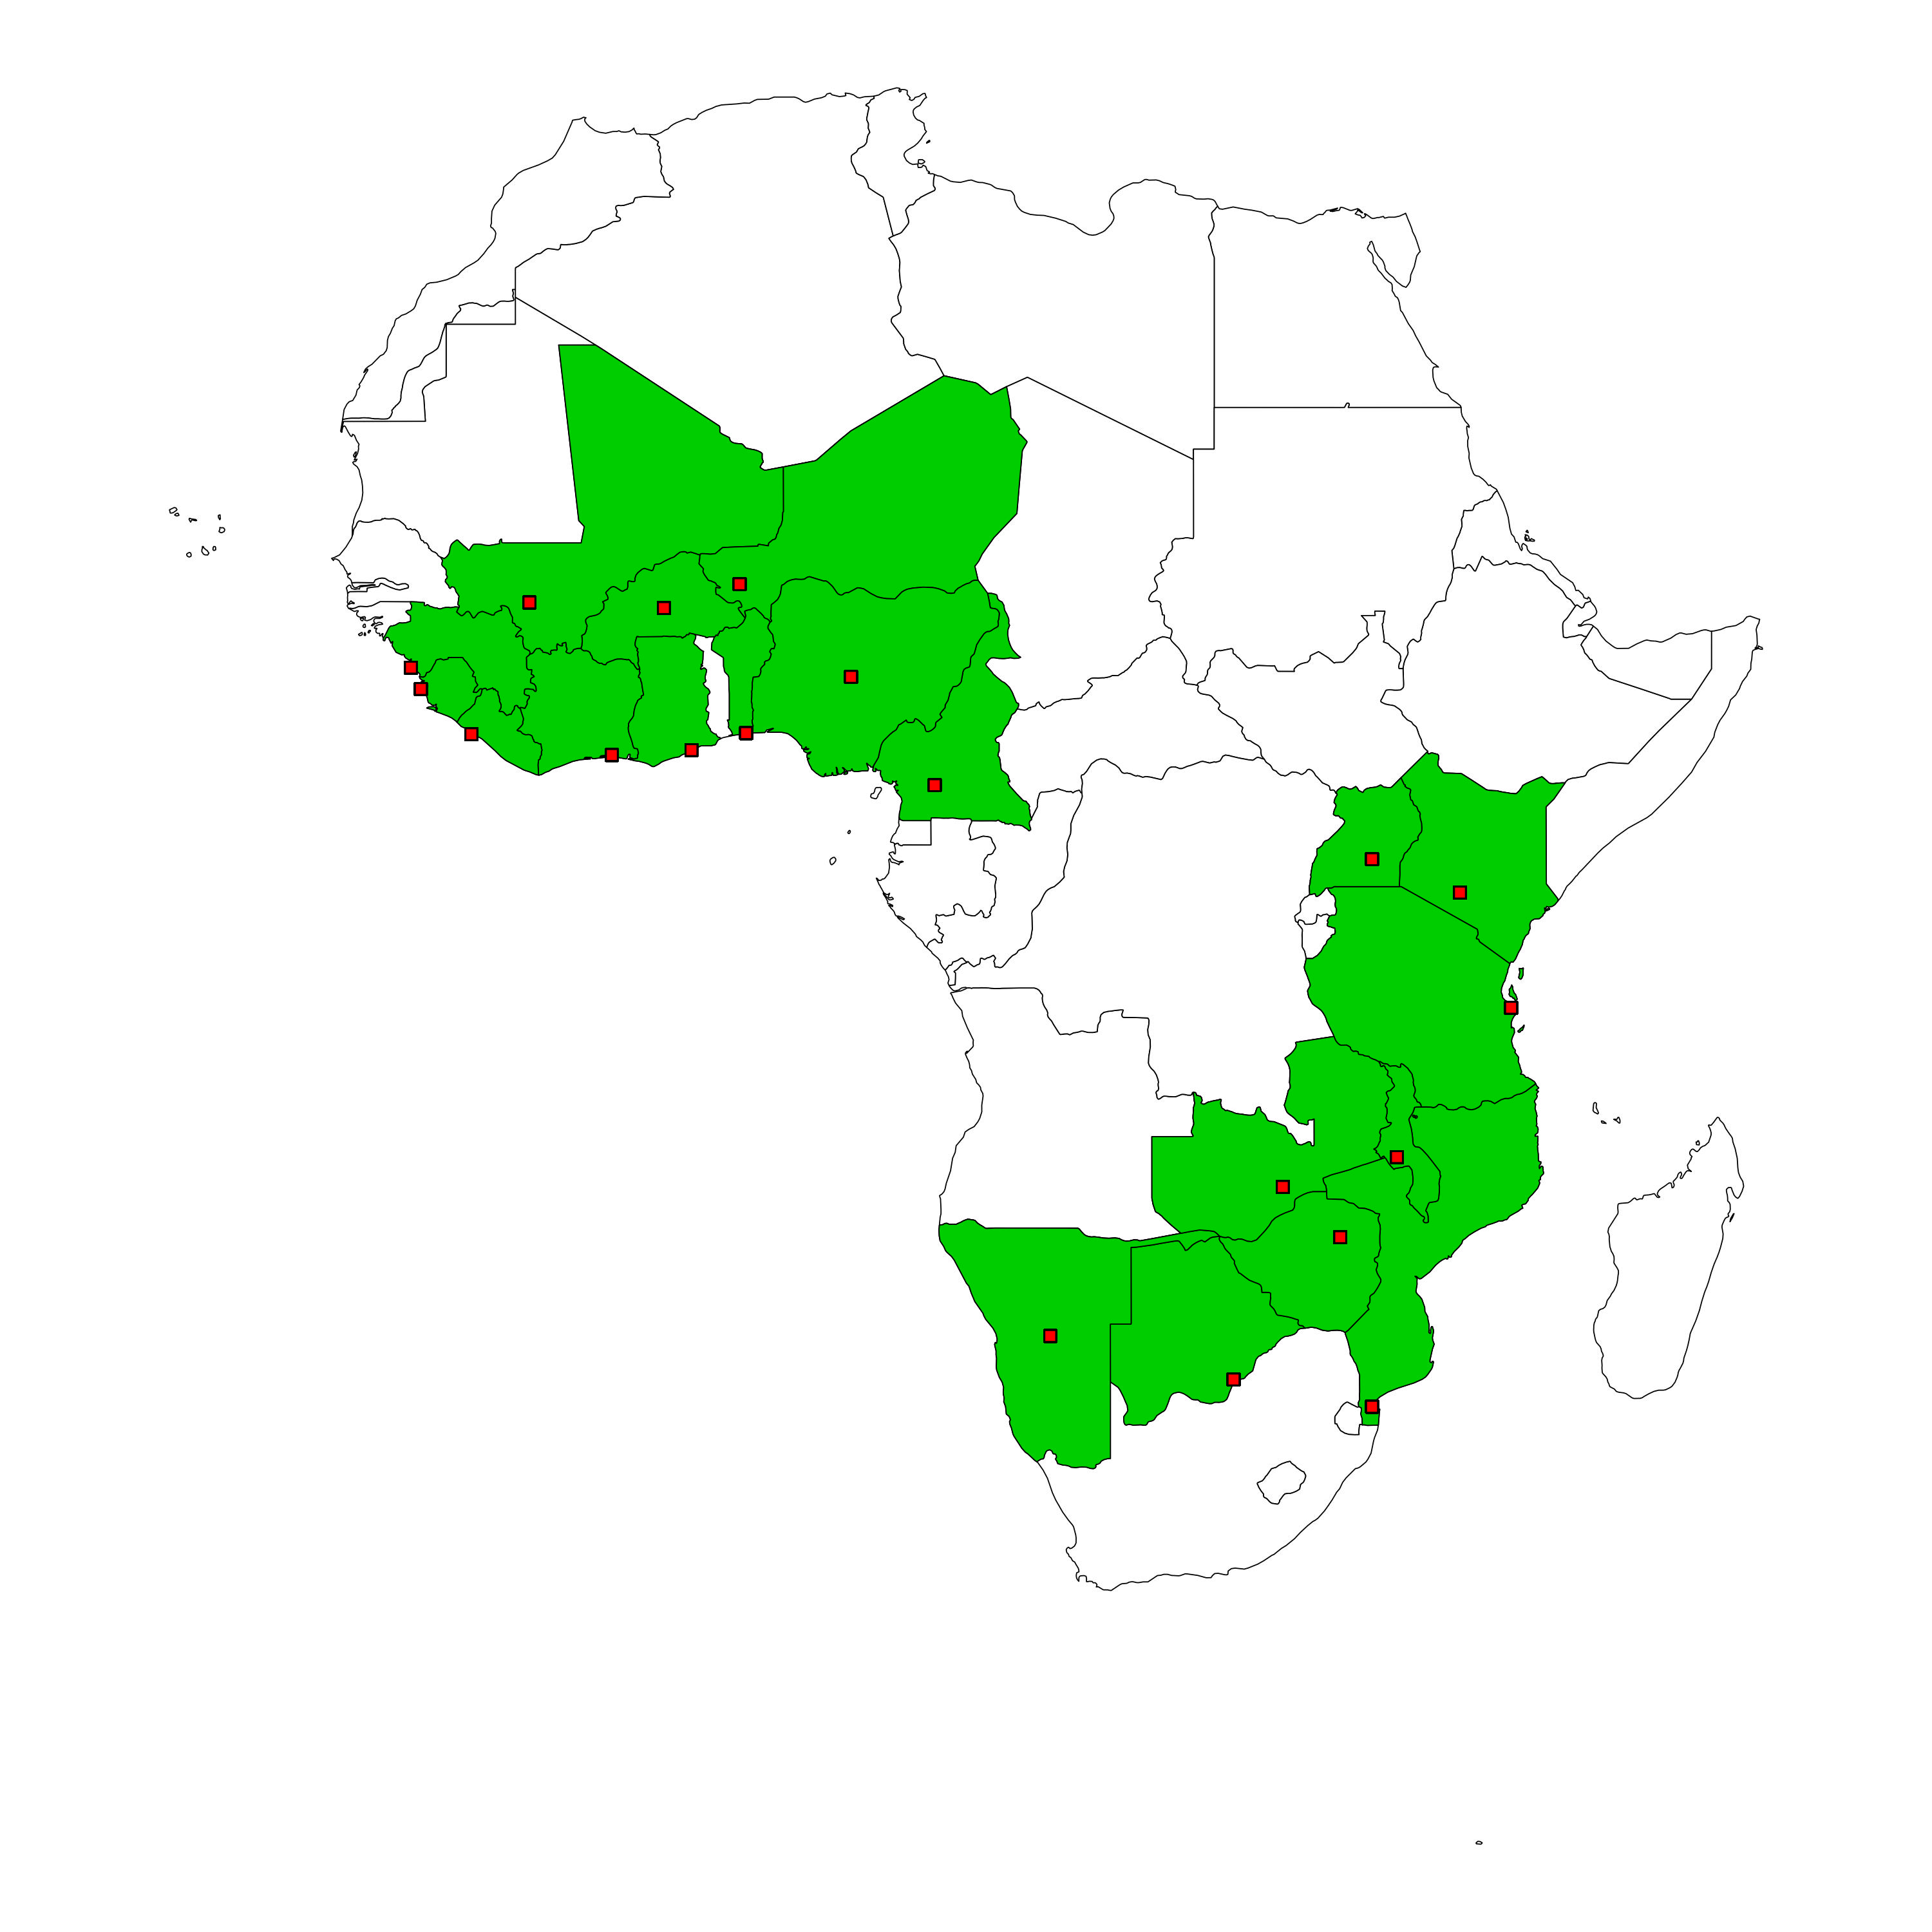
\includegraphics[width=6cm]{C:/Users/Redha CHABA/Documents/working_paper/trust/plots/map/obs_map.jpg}
    \end{figure}
    \end{column}
        \end{columns}
    \end{frame}


\begin{frame}{Empirical strategy - Distance and political trust}
    \centering \textbf{Effect of distance from the capital city on political trust}\vspace{1em}
        \begin{equation}
        trust_{irct} = \beta_{0} + \beta_{1}dist_{irc} + \Gamma X^{'}_{ir} + \mu_{ct} + \varepsilon_{irct}
        \end{equation}
        \begin{itemize}\setlength\itemsep{1em}

            \item $trust_{irct}$: Average trust in parliament and president \vfill
            \item $dist_{irc}$: Normalized distance from the capital \\
            \textcolor{gray}{\textit{Michalopoulos and Papaioannou, 2014}}\vfill
            \item $X^{'}_{ir}$: Individual and regional controls\vfill
            \item $\mu_{ct}$: Country $\times$ round fixed effects\vfill
            \item $\varepsilon_{irct}$: Error term\vfill
            \item Robust standard errors clustered at the region x round level
        \end{itemize}
\end{frame}

\begin{frame}{Empirical strategy - Distance and political trust}
    \begin{figure}
        \centering
        \caption{Historical Ethnic Areas and Contemporary National Boundaries}
        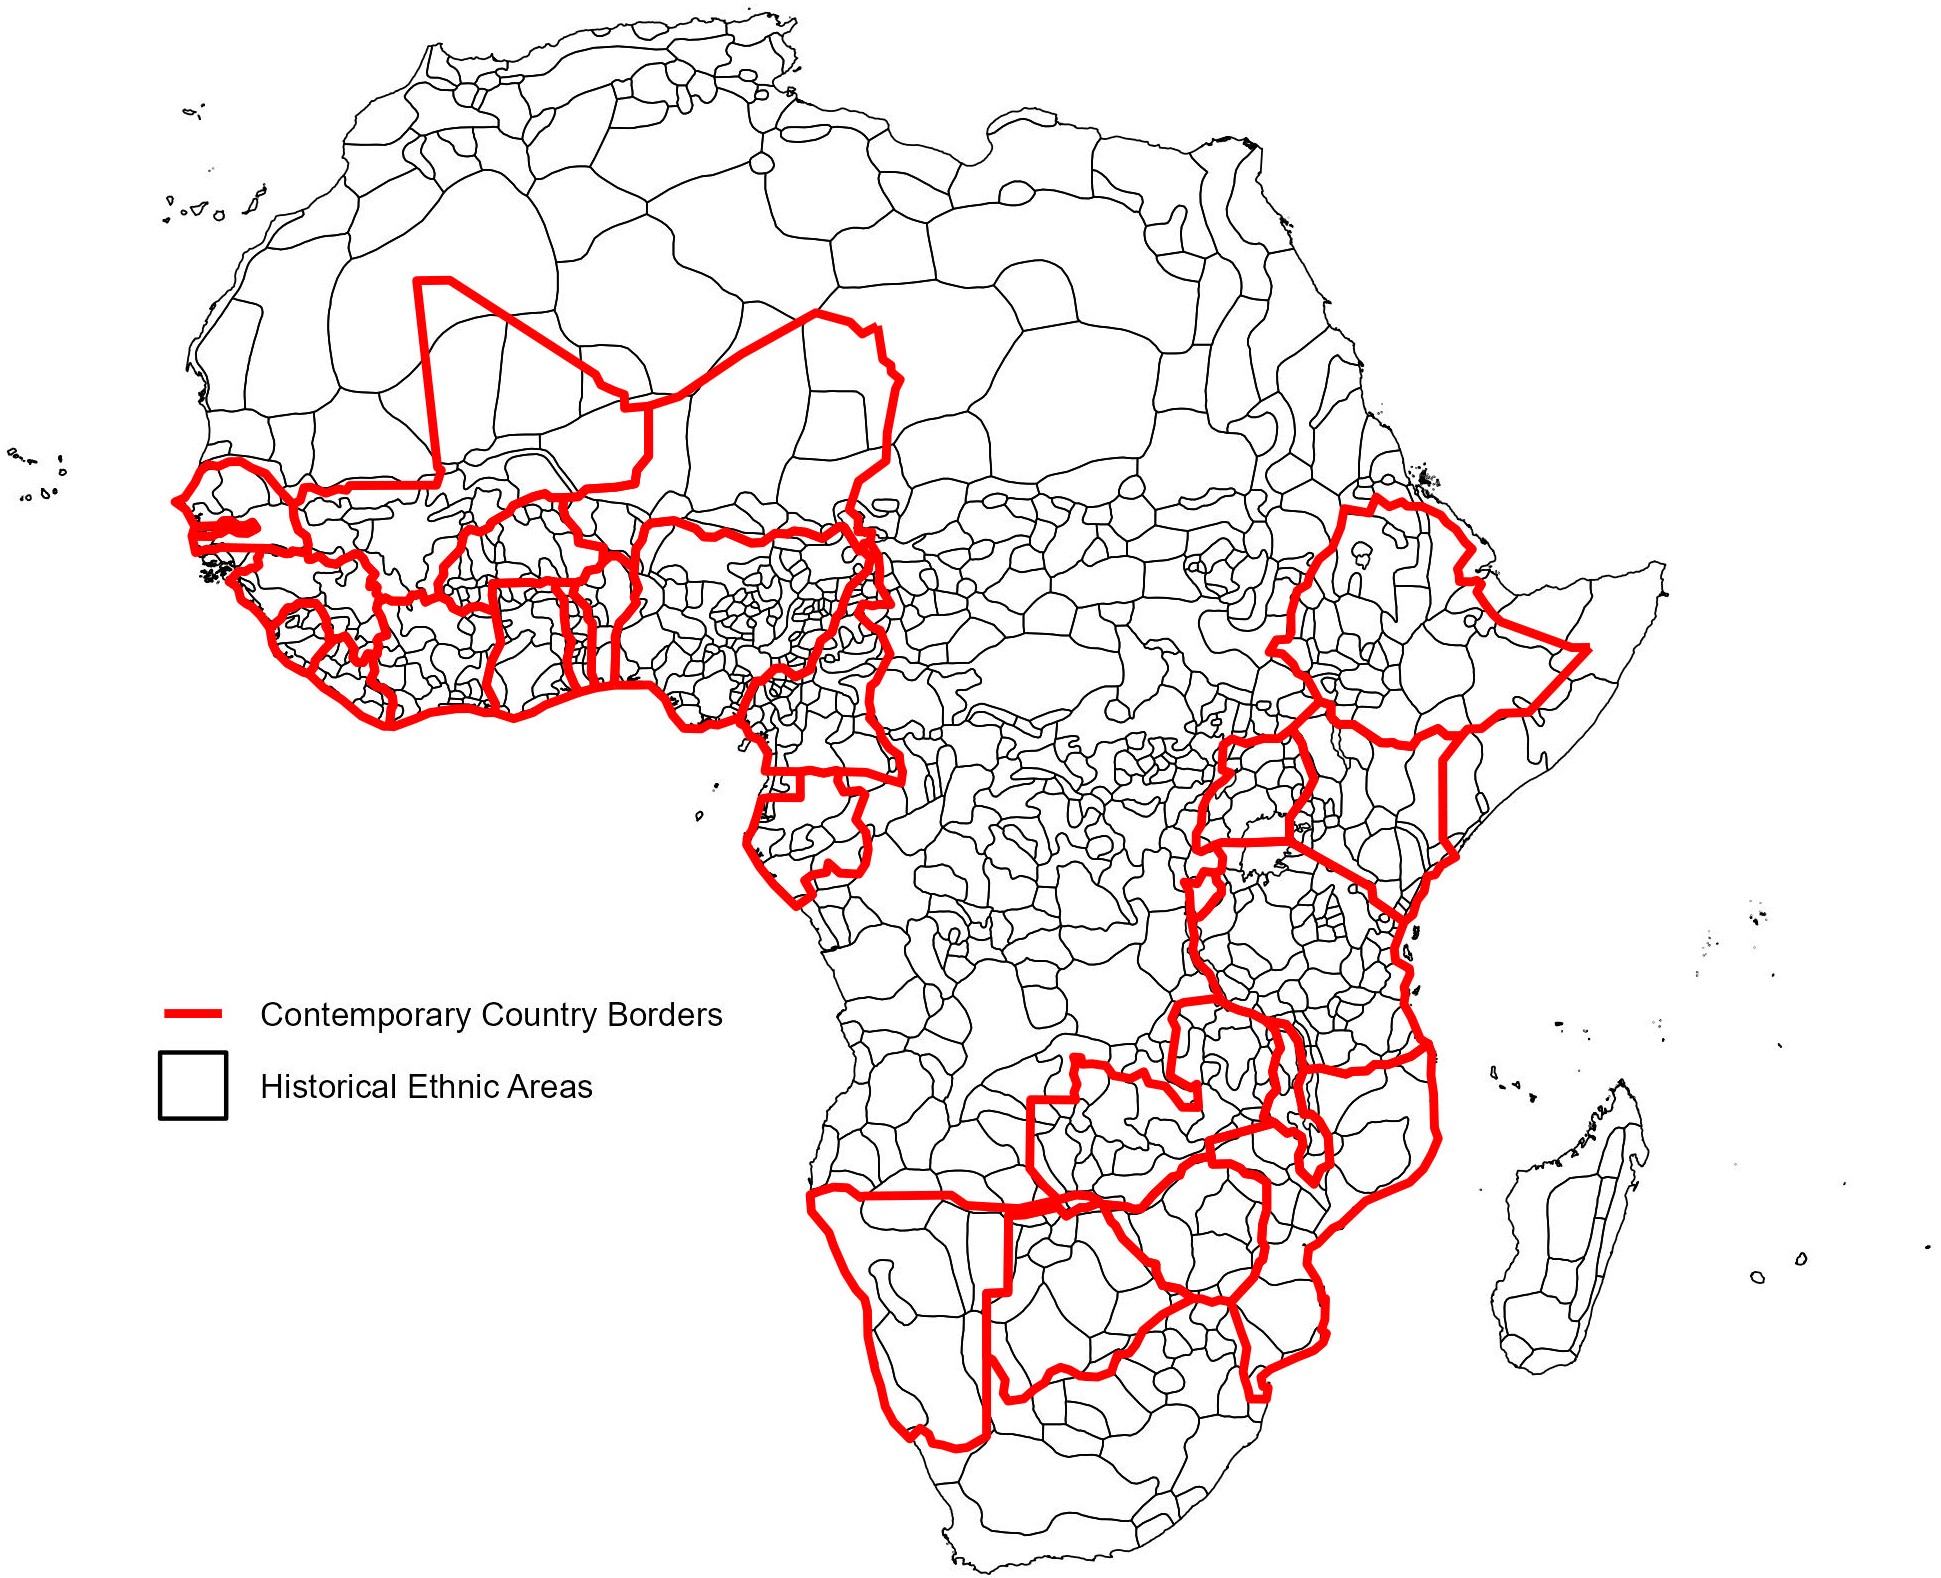
\includegraphics[width=8cm]{murdock_map.jpg}
    \end{figure}
    
\end{frame}


\begin{frame}{Empirical strategy - Distance and political trust}

    \begin{figure}
        \centering
        \caption{Exemple: Dendi Ethnic Group}
        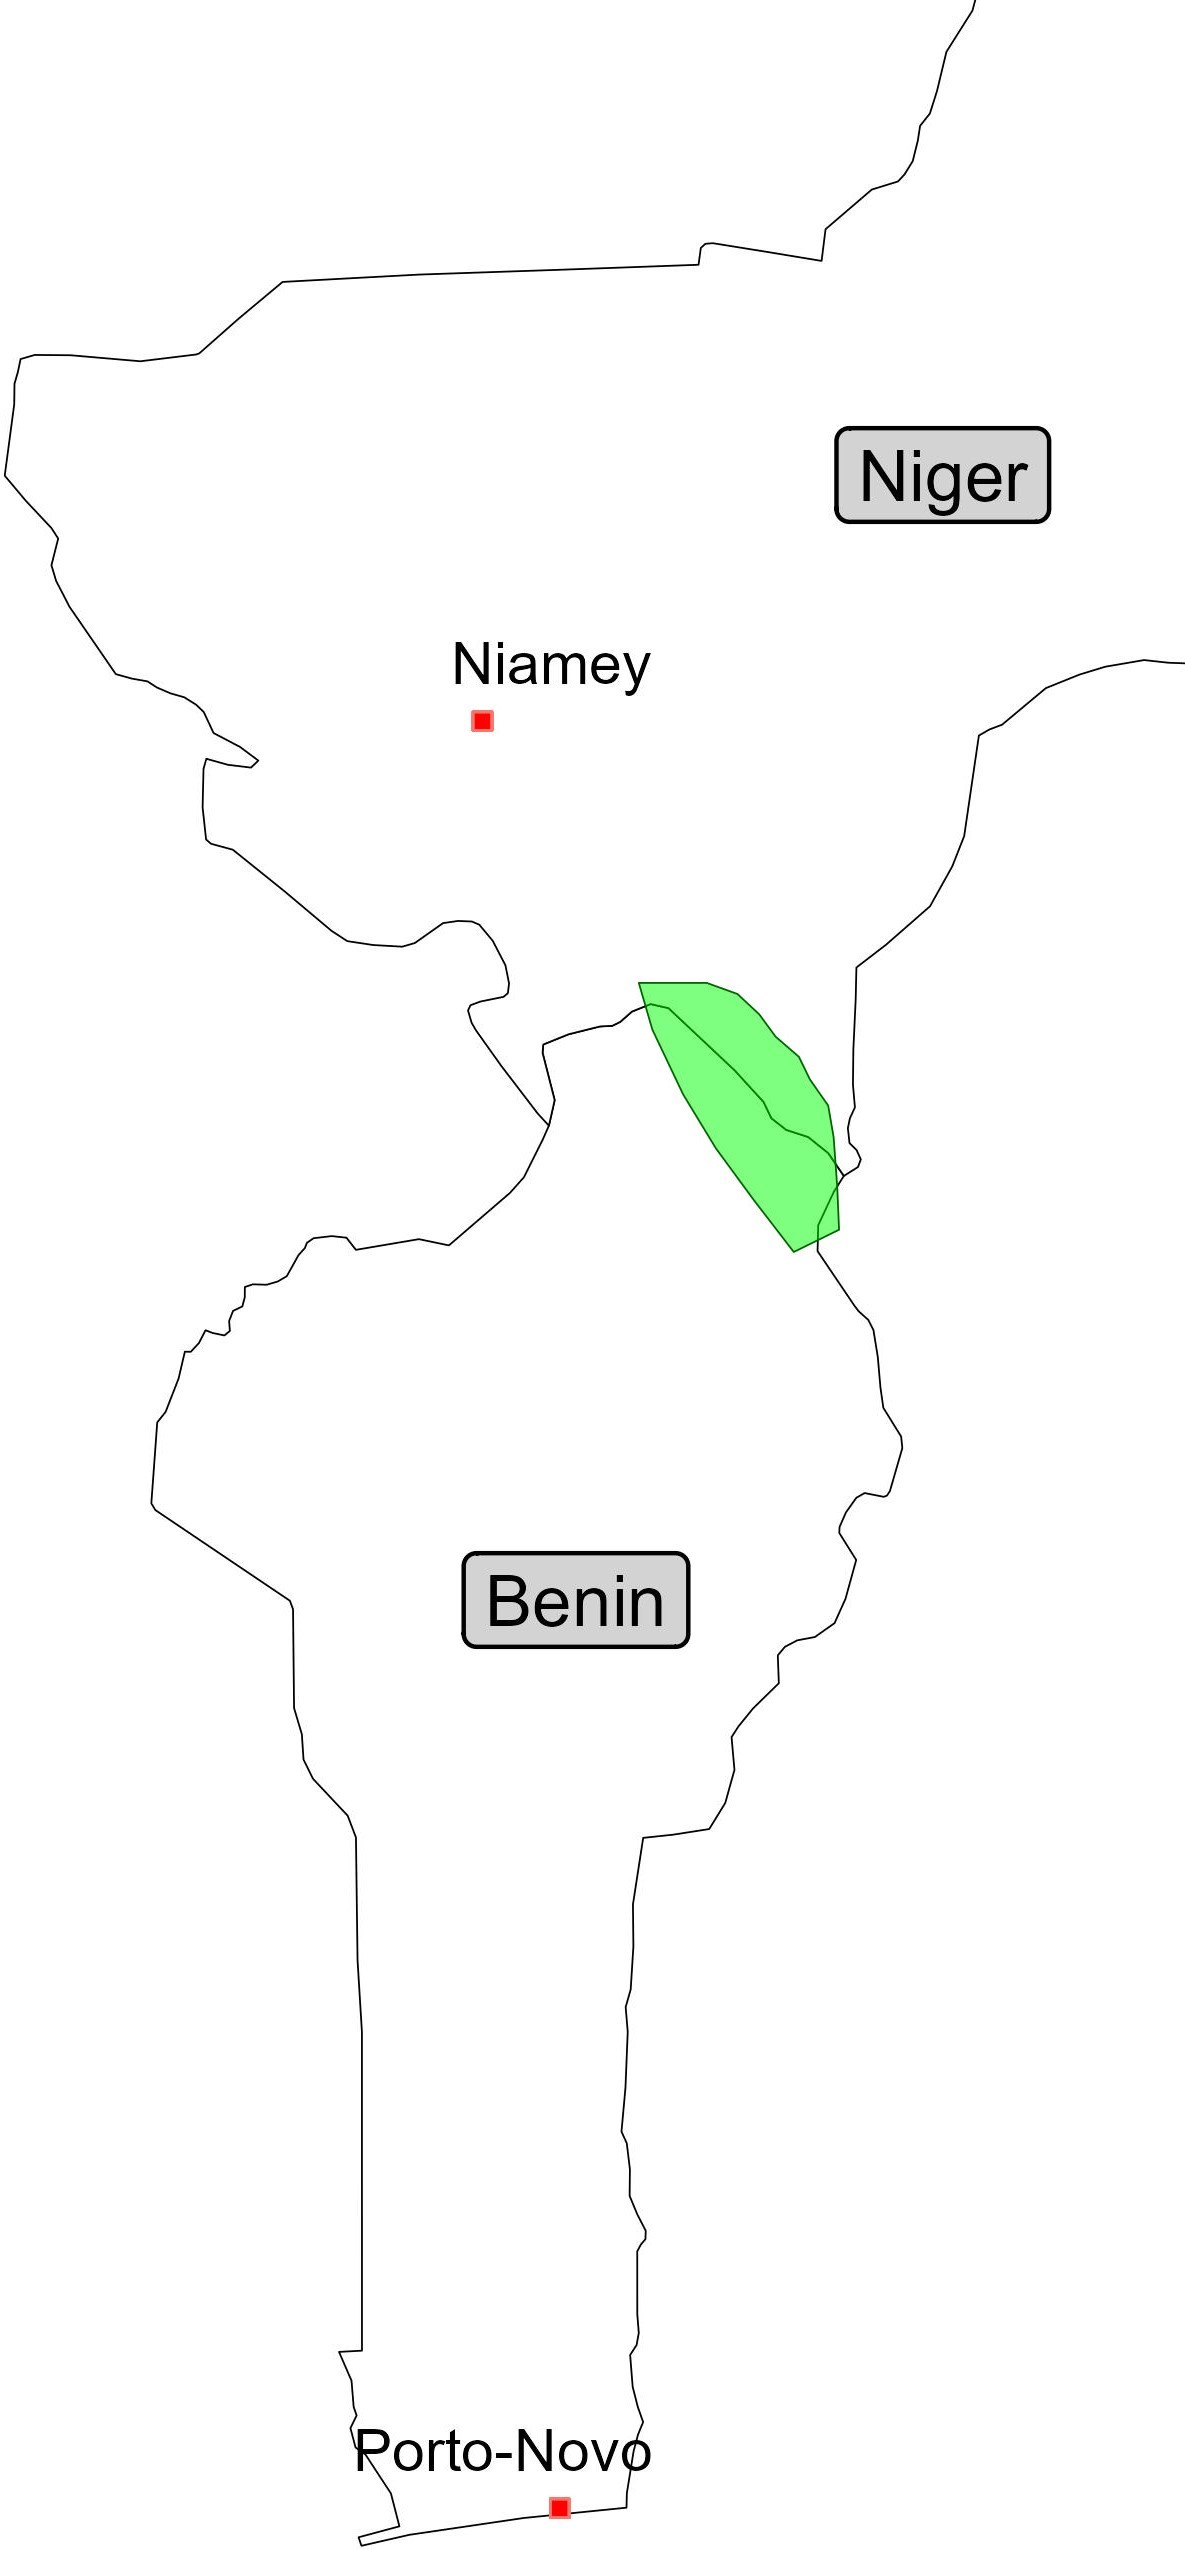
\includegraphics[width=2.8cm]{bdd_map.jpg}
    \end{figure}

\begin{equation}
trust_{irct}=\beta_{0}+\beta_{1}dist_{irc}+\Gamma X^{'}_{ir}+\textcolor[rgb]{0.0,0.6,0.0}{\mathbf{\nu_{e}}}+\mu_{ct}+\varepsilon_{irct}
\end{equation}

\end{frame}


\begin{frame}{Empirical strategy - Distance and political trust}
    \centering \textcolor{rougeprez}{\textbf{Identification assumptions}}\vfill
    \setbeamertemplate{enumerate items}[default]
    \begin{enumerate}
        \item Two individuals living in the same historical ethnic region share similar geographical, social, and historical traits, except for their distance from the capitals\vfill
        \item The differences observed on either side of the country border are not attributable to institutional differences\vfill
        
\begin{equation}
    trust_{irct}=\beta_{0}+\beta_{1}dist_{irc}+\Gamma X^{'}_{ir}+ \textcolor[rgb]{0.0,0.6,0.0}{\theta Z^{'}_{ct}} + \textcolor[rgb]{0.0,0.6,0.0}{\mathbf{\nu_{e}}}+\textcolor[rgb]{0.0,0.6,0.0}{\lambda_{t}}+\varepsilon_{ict}
    \end{equation}
            
    \end{enumerate}
\end{frame}







\begin{frame}{Distance increases political trust}

    \begin{table}[H]
        \sffamily
        \caption{{Effect of distance from the capital on political trust}}
        \centering
        %\footnotesize
        \resizebox{8cm}{!}{
        \begin{tabular}{@{\extracolsep{5pt}} l c c c c}
        \\
        \toprule
        \toprule
        &  \multicolumn{4}{c}{{OLS}}  \\
        \cmidrule(r){2-5}
        &  \multicolumn{4}{c}{{Political trust}}  \\
        \cmidrule(r){2-5}
        & \multicolumn{2}{c}{{Base sample}} & \multicolumn{2}{c}{{Border sample}}\\
            \cmidrule(r){2-3}
            \cmidrule(r){4-5}
            & \multicolumn{1}{c}{{(1)}} &  \multicolumn{1}{c}{{(2)}}  & \multicolumn{1}{c}{{(3)}} &  \multicolumn{1}{c}{{(4)}}\\
         \midrule
      
         Distance from the capital&       0.300***&       0.298***&       0.618***&       0.341** \\
         \smallskip
         &      (0.04)   &      (0.03)   &      (0.15)   &      (0.16)   \\
         \midrule
         \smallskip
        Individual \& regional controls  & Yes & Yes & Yes & Yes  \\
        \smallskip
        Country controls & Yes& No& Yes& No\\
        \smallskip
        Round FE & Yes & No& Yes & No\\
        \smallskip
        Country X Round FE       & No & Yes& No & Yes\\
        \smallskip
        Ethnic homeland FE & No & No & Yes& Yes\\
        \smallskip
        Observations           &      107,117   &      111,570   &       10,790   &       11,924   \\
        Adjusted-R$^2$         &       0.105   &       0.156   &       0.140   &       0.172   \\
                              \bottomrule
        \multicolumn{5}{p{12.5cm}}{\footnotesize \emph{Notes}: The border sample includes individuals residing within a 40-kilometer buffer around a country border that overlaps with a historical ethnic homeland, as defined by Murdock (1959). Robust standard errors clustered at the region x round level  for the base sample and ethnic homeland x region x round level for the border sample are in parentheses. The set of individual controls
        includes measures of: normalized distance from the largest non-capital city, age, age squared, sex,
        education, employment status, rural/urban situation, personal economic conditions perception, interest in politics, TV news consumption, radio news consumption, newspaper consumption. (3) and (4) also include a measure of ethnic discrimination. The set of regional controls includes measures of: nighttime light, population density, region area, president birthplace dummy. The set of country controls includes: log(GDP.p.c.), log(area), V-Dem Polyarchy index, World Bank corruption index, political regime type, colonial origin. *** / ** / * represent significance at the 0.01 / 0.05 / 0.10 levels, respectively.}
        \end{tabular}
        }
        \end{table}
        \end{frame}

\begin{frame}{Distance increases political trust}

\begin{figure}
    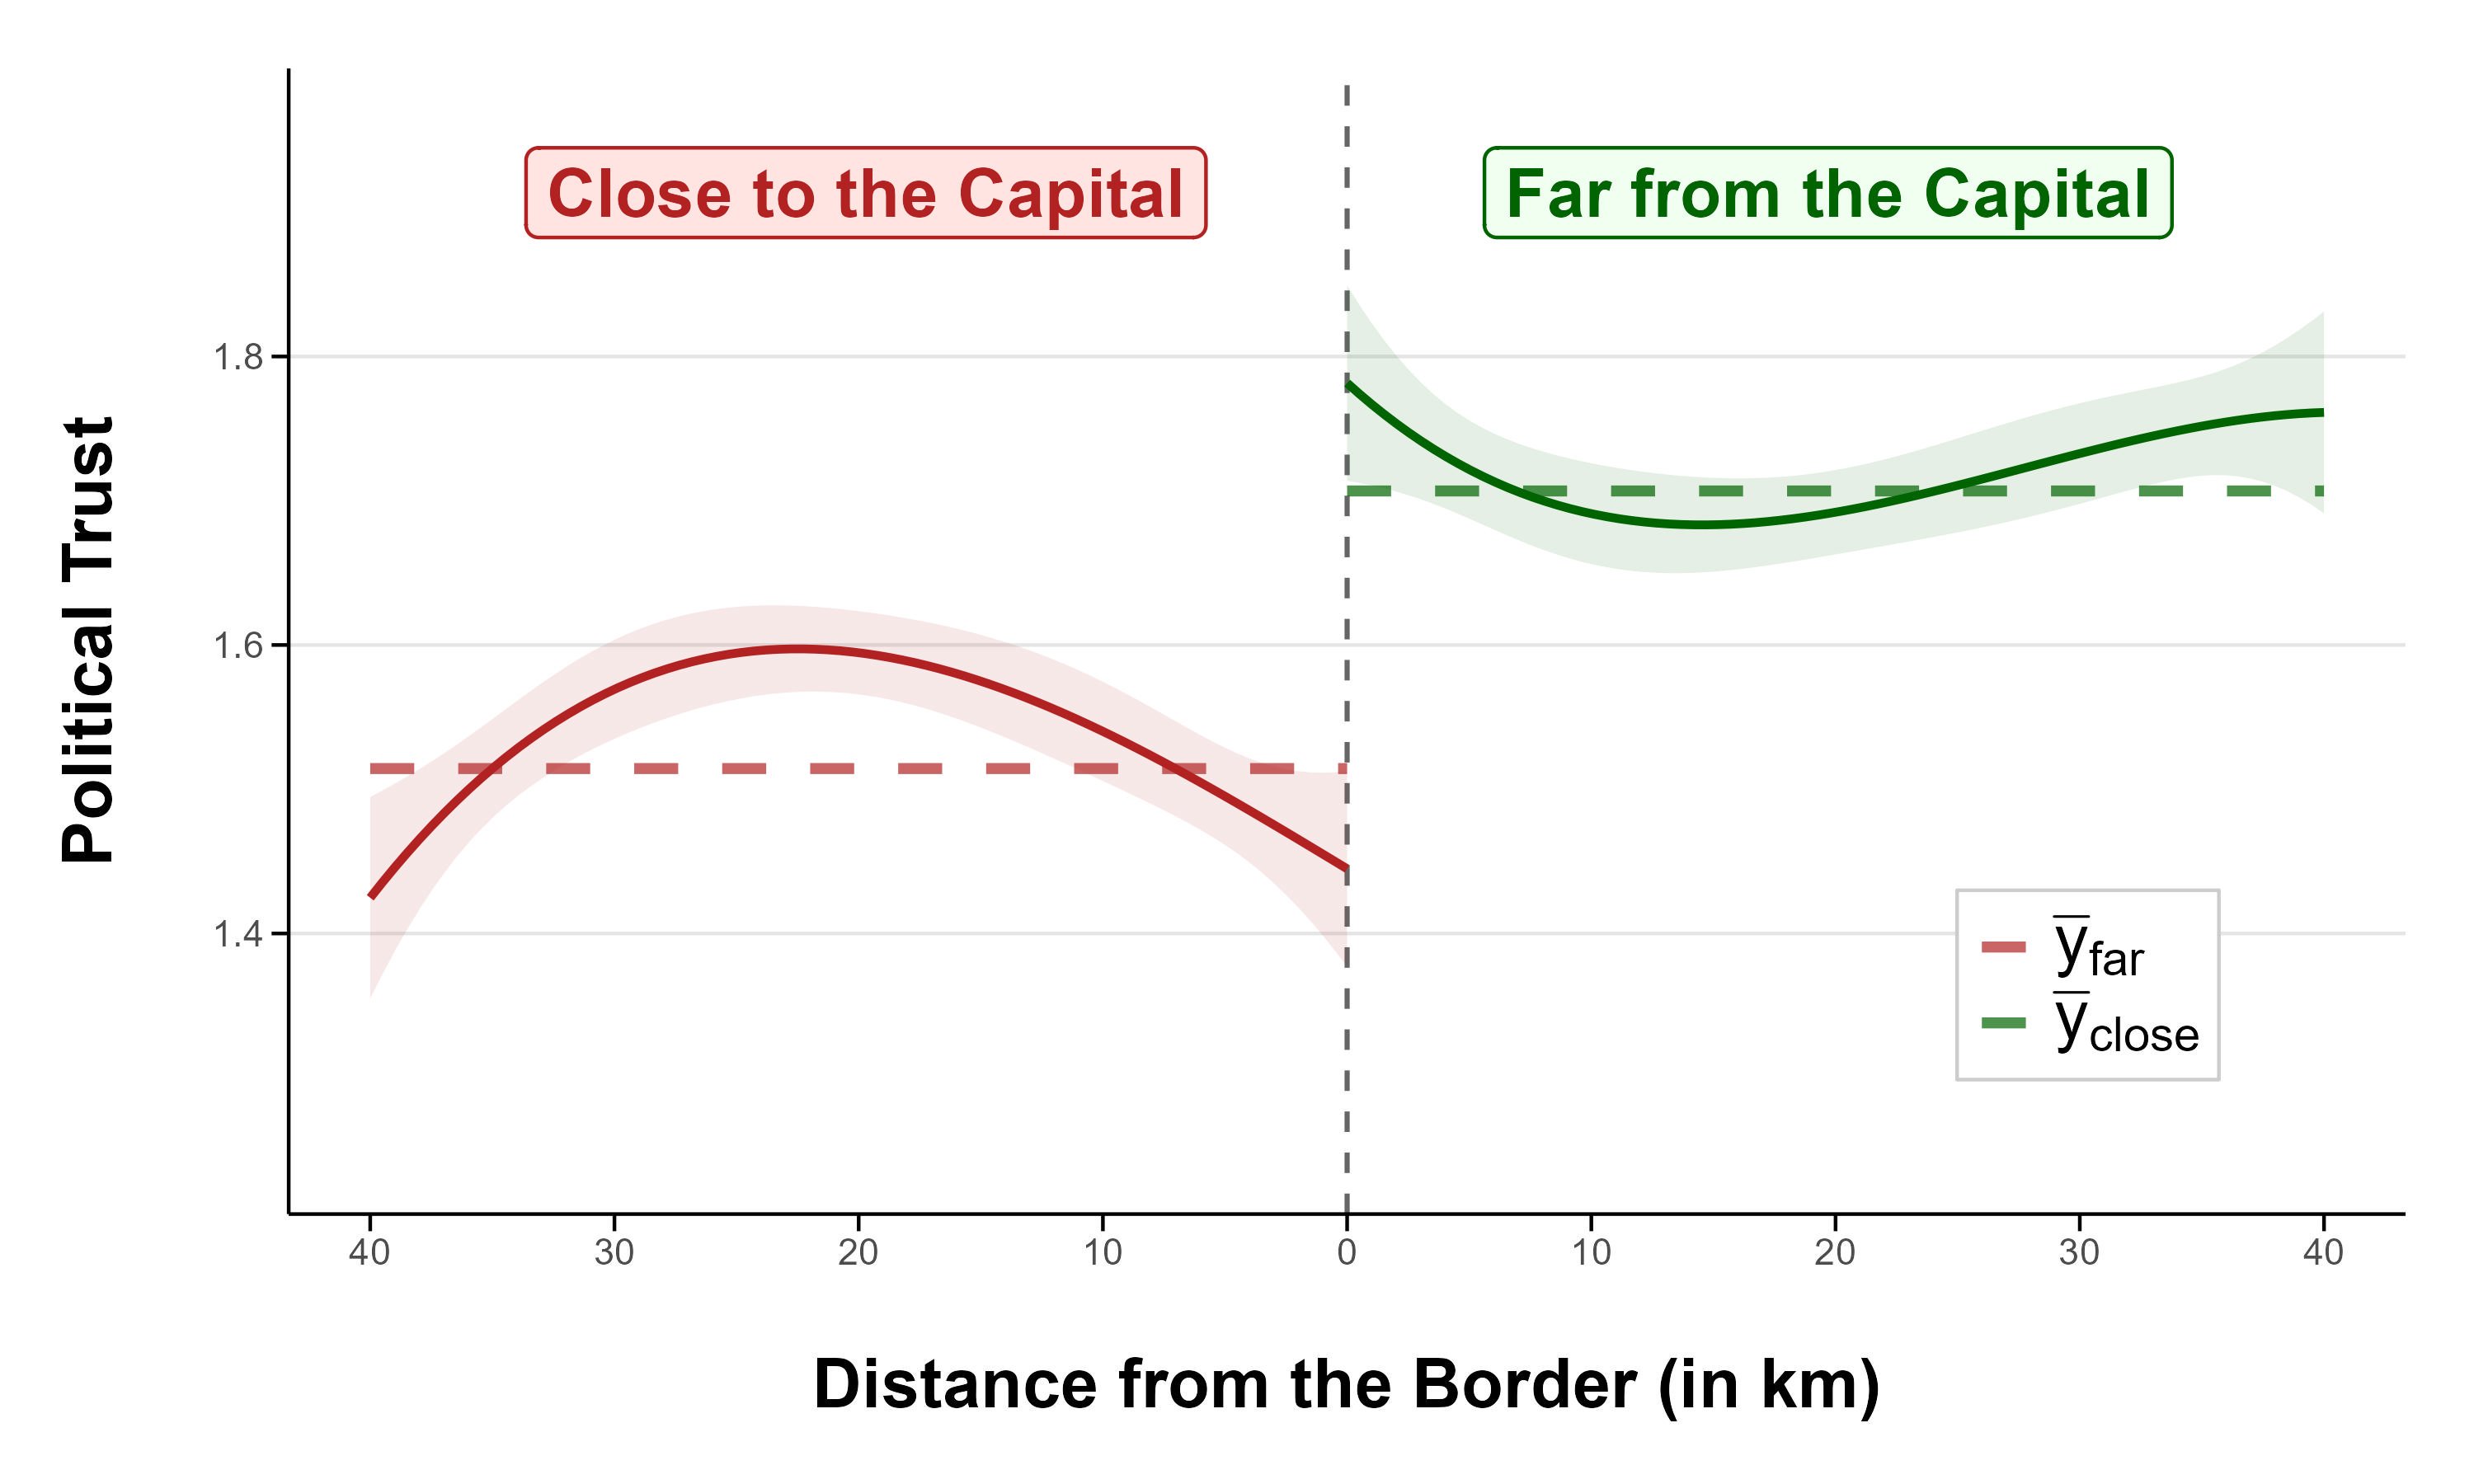
\includegraphics[scale=0.1]{C:/Users/Redha CHABA/Documents/working_paper/trust/plots/discontinuity/discontinuity.jpg}
    \caption{Border discontinuity - \textit{Based on regression estimates from (3) of Table 1}}
\end{figure}

\end{frame}


\begin{frame}{{\fontsize{13}{12}\selectfont
    Empirical strategy - Internet coverage and spatial patterns of opinion}}
\centering \textcolor{rougeprez}{\textbf{Effect of internet coverage on political trust by distance}}\vspace{1em}

\begin{equation}
    \fontsize{8}{10}\selectfont
\begin{split}
trust_{irct} = & \beta_{0} + \beta_{1} dist_{irc} + \beta_{2} \textcolor{red}{\textbf{internet\_coverage}_{irct}} + \beta_{3} \textcolor{red}{\textbf{dist} \times \textbf{internet\_coverage}_{irct}} \\
& + \Gamma X^{'}_{ir} + \mu_{ct}+ \varepsilon_{irct}
\end{split}
\end{equation}\vspace{1em}

\noindent
{\fontsize{9}{12}\selectfont
\textcolor{red}{\textbf{internet\_coverage}$_{irct}$:} Regional average of internet coverage weighted by population density \textcolor{gray}{\textit{Guriev et al., 2021, Cariolle and Carroll, 2024}}
}
\vfill

\begin{itemize}\setlength\itemsep{1em}

    \item \textcolor{red}{\textbf{Reverse causality:}} Areas with higher political trust might experience less deployment of internet infrastructure
\end{itemize}
\end{frame}

\begin{frame}{{\fontsize{13}{12}\selectfont
    Empirical strategy - Internet coverage and spatial patterns of opinion}}
    \begin{figure}
        \centering
        \caption{Example: Benin Lightning strike and Internet Coverage}
        
        \begin{subfigure}{0.45\textwidth}
            \centering
            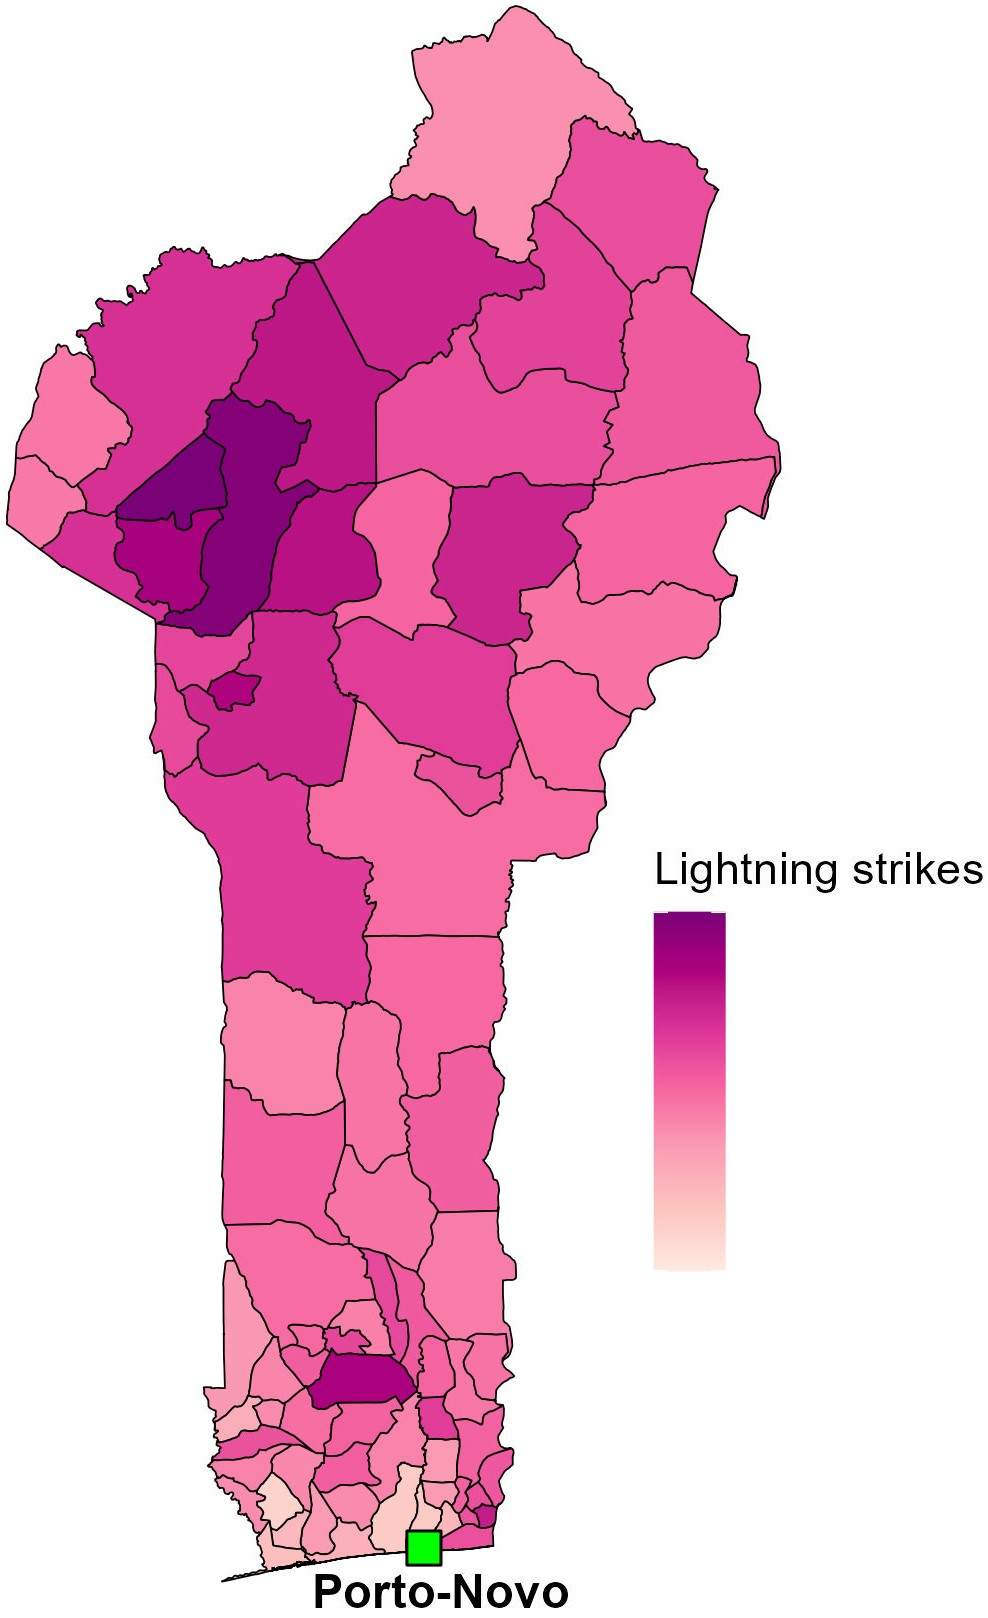
\includegraphics[width=3.8cm]{lightning_strikes.jpg}
            \caption{Lightning strike}
        \end{subfigure}
        \hspace{0.02\textwidth}
        \begin{subfigure}{0.45\textwidth}
            \centering
            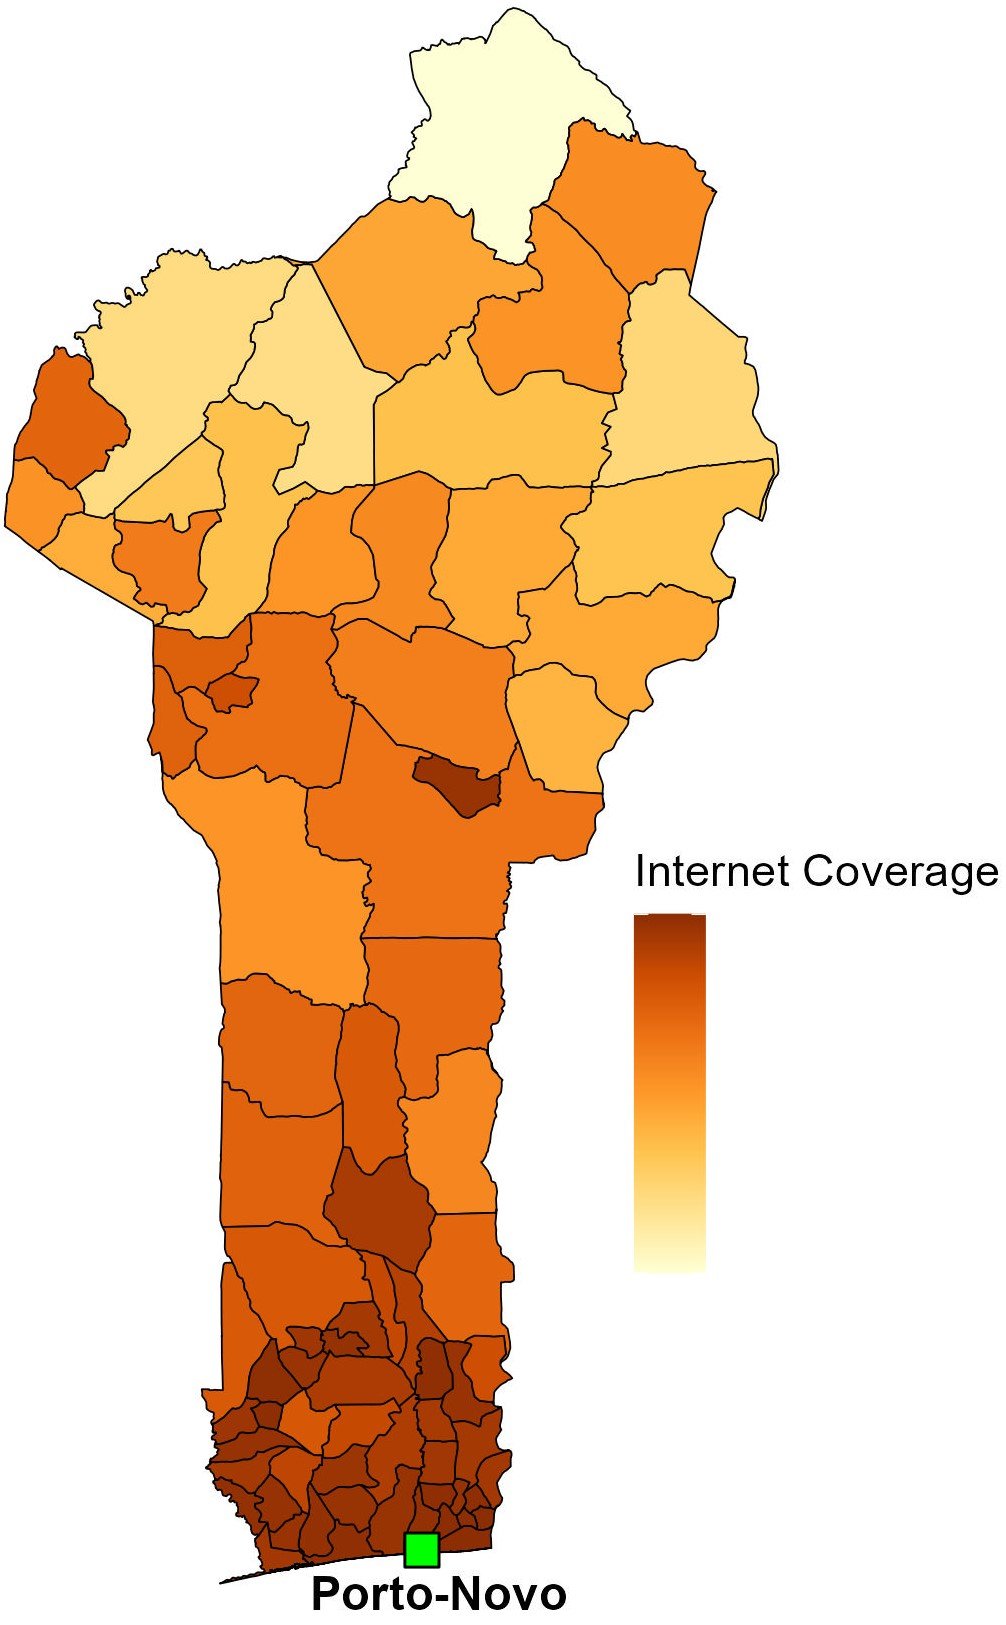
\includegraphics[width=3.8cm]{internet_coverage_w8.jpg}
            \caption{Internet coverage (2020)}
        \end{subfigure}        
    \end{figure}
\end{frame}

\begin{frame}{{\fontsize{13}{12}\selectfont
    Empirical strategy - Internet coverage and spatial patterns of opinion}}    
    \centering \textcolor{rougeprez}{\textbf{Lightning strike instrument}}
    \vspace{1.5em}
    \begin{itemize}\setlength\itemsep{1em}
\setlength\itemsep{1em}
        \item Instrument internet coverage
        using regional lightning strike patterns \textcolor{gray}{\textit{Manacorda and Tesei, 2020; Guriev
                et al., 2021; Cariolle and Carolle, 2024}}\vfill
        \item Areas with frequent lightning strike face higher infrastructure deployment and maintenance costs, while these weather patterns
                are plausibly exogenous to political trust\vfill
        \item Average daily lightning strike at the regional level using VHRFC data over 1998-2013, weighted by population density\vfill
    \end{itemize}
    \vspace{1em}

\centering \textcolor{rougeprez}{\textbf{Geographical instrument $\rightarrow$ focus on the base sample}}
\end{frame}

\begin{frame}{{\fontsize{13}{12}\selectfont
    Empirical strategy - Internet coverage and spatial patterns of opinion}}
    \centering \textbf{First-stage}

    \begin{equation}
        \begin{split}
            \textcolor{red}{\textbf{internet\_coverage}_{irct}} = & \beta_{0} + 
            \beta_{1} \textcolor[rgb]{0.0,0.6,0.0}{\textbf{lightning\_strike}_{r} \times t} + \Gamma X^{'}_{ir} \\
            & \quad + \mu_{ct}+ v_{irct}
        \end{split}
        \end{equation}\\
    
    \begin{equation}
    \begin{split}
        \textcolor{red}{\textbf{dist} \times \textbf{internet\_coverage}_{irct}} = & \beta_{0} + 
        \beta_{1} \textcolor[rgb]{0.0,0.6,0.0}{\textbf{dist} \times \textbf{lightning\_strike}_{r} \times t} + \Gamma X^{'}_{ir} \\
        & \quad + \mu_{ct}+ v_{irct}
    \end{split}
    \end{equation}\\

    \centering \textbf{Second-stage}
    \fontsize{8}{10}\selectfont
    \begin{equation}
        \begin{split}
        trust_{irct} = & \beta_{0} + \beta_{1} dist_{irc} + \beta_{2}^{2S}\textcolor[rgb]{0.0,0.6,0.0}{\textbf{internet\_coverage}_{irct}} + \beta_{3}^{2S}\textcolor[rgb]{0.0,0.6,0.0}{\textbf{dist} \times \textbf{internet\_coverage}_{irct}} \\
        & + \Gamma X^{'}_{ir} + \mu_{ct}+ \varepsilon_{irct}
        \end{split}
        \end{equation}        
    
\end{frame}





\begin{frame}{Internet mitigates spatial patterns of opinion}
    \begin{table}[H]
        \sffamily
        \caption{Effect of internet coverage on political trust by distance}
        \centering
        %\footnotesize
        \resizebox{12cm}{!}{
        \begin{tabular}{@{\extracolsep{5pt}} l c c c c c c}
        \\
        \toprule
        \toprule
        & \multicolumn{5}{c}{{Base sample}}\\
        \cmidrule(r){2-6}
        & \multicolumn{1}{c}{{OLS}} & \multicolumn{3}{c}{{First Stage}} & \multicolumn{1}{c}{{2SLS}}\\
            \cmidrule(r){2-2}
            \cmidrule(r){3-5}
            \cmidrule(r){6-6}
            & \multicolumn{1}{c}{{Political trust}} & \multicolumn{1}{c}{{Internet coverage}} & \multicolumn{1}{c}{{}} &  \multicolumn{1}{c}{{Distance $\times$ Internet coverage}} & \multicolumn{1}{c}{{Political trust}}\\
            \cmidrule(r){2-2}
            \cmidrule(r){3-3}
            \cmidrule(r){5-5}    
            \cmidrule(r){6-6}    
            & \multicolumn{1}{c}{{(1)}} & \multicolumn{1}{c}{{(2)}} & \multicolumn{1}{c}{{}} &  \multicolumn{1}{c}{{(3)}} & \multicolumn{1}{c}{{(4)}}\\
            
            \midrule
      
    
    Distance from the capital&       0.453***&&&&       1.523***\\
    \smallskip
    &      (0.05)   &&&&      (0.56)   \\
    Internet coverage&      -0.015   &&&&       1.770** \\
\smallskip
&      (0.06)   &&&&      (0.69)   \\
Distance from the capital $\times$ Internet coverage&     -0.466***&&&&       -2.950**         \\
\smallskip
            &      (0.10)   &&&&        (1.45)           \\


   Lightning strikes && -0.002*** && -0.000  \\
    \smallskip&& (0.00) && (0.00) \\
    Distance from the capital city $\times$ Lightning strikes&&-0.000 && -0.001***\\
    \medskip&& (0.00) && (0.00)\\
    
         \midrule
        SW \emph{F} - Lightning strikes &-&-& 13.74&- &-\\
        \smallskip
        SW \emph{F} - Distance $\times$ Lightning strikes &-&-& 8.62 &-&-\\
        \smallskip
        Individual \& regional controls  & Yes & Yes &&  Yes & Yes\\
        \smallskip
        Country X Round FE       & Yes & Yes&- & Yes & Yes \\
        \smallskip
        Observations       &       111,570    &113,243 & 113,243&       111,570  \\
        Adjusted-R$^2$    &       0.158     &-&-&-&  \\
                              \bottomrule
        \multicolumn{6}{p{25cm}}{\footnotesize \emph{Notes}: % Set font size to 8pt with 10pt line spacing
        \emph{Notes}: Robust standard errors clustered at the region x round level. The set of individual controls
        includes measures of: normalized distance from the largest non-capital city, age, age squared, sex,
        education, employment status, rural/urban situation, personal economic conditions perception, ethnic discrimination, interest in politics, TV news consumption, newspaper consumption, radio consumption. The set of regional controls includes measures of: nighttime light, population density, region area, president birthplace dummy. *** / ** / * represent significance at the 0.01 / 0.05 / 0.10 levels, respectively.}
    \end{tabular}}
        \end{table}
\end{frame}

\begin{frame}{Internet mitigates spatial patterns of opinion}

    
\begin{figure}
    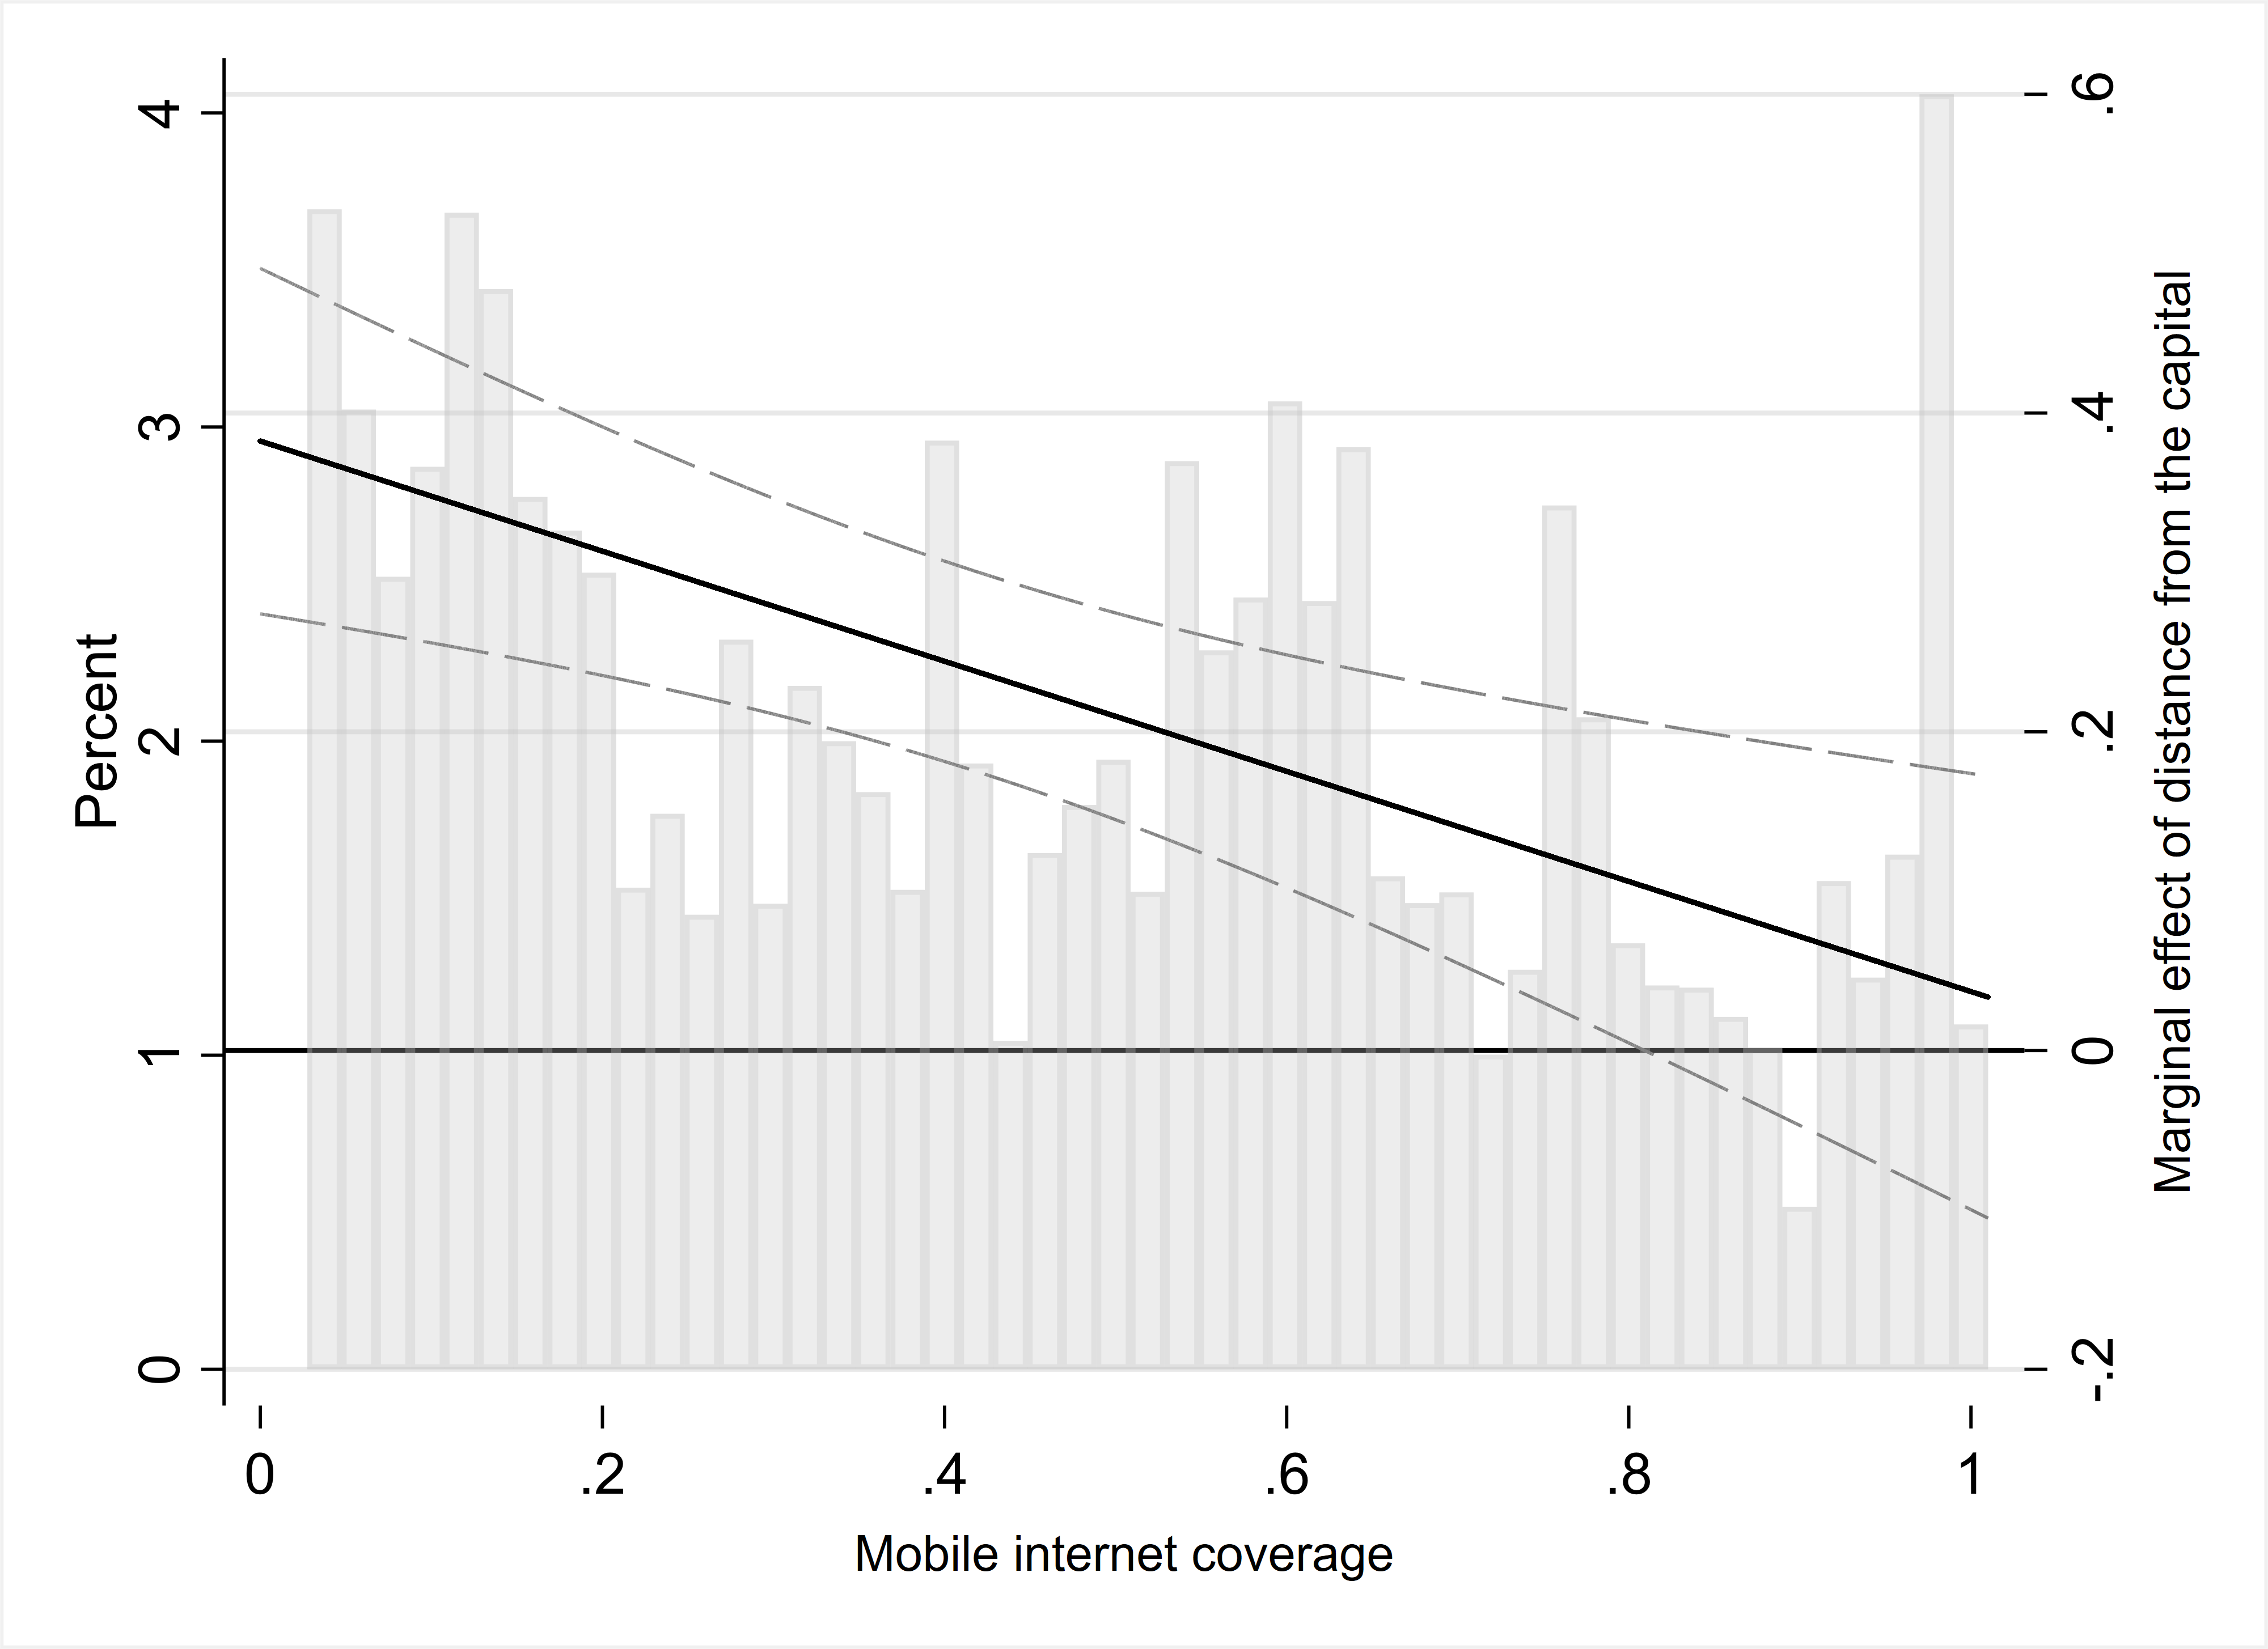
\includegraphics[scale=0.07]{C:/Users/Redha CHABA/Documents/working_paper/trust/plots/marginal_effect/pol_trust.png}
    \caption{Marginal effect of Distance from the capital as a function of Internet coverage}
\end{figure}

\end{frame}


\begin{frame}{Internet is effective in countries with weak institutions}
    \begin{table}[H]
        \sffamily
        \caption{{Media and institutions freedom}}
        \centering
        %\footnotesize
        \resizebox{10.5cm}{!}{
        \begin{tabular}{@{\extracolsep{5pt}} l c c c c}
        \\
        \toprule
        \toprule
        & \multicolumn{4}{c}{2SLS: Political trust}\\
        \cmidrule(r){2-5}
        & \multicolumn{4}{c}{{Base sample}}\\
        \cmidrule(r){2-5}
        &\multicolumn{2}{c}{{Media}}&  \multicolumn{2}{c}{{Institutions}}\\
        \cmidrule(r){2-3}
            \cmidrule(r){4-5}
            & \multicolumn{1}{c}{{Free}} & \multicolumn{1}{c}{{Captured}}& \multicolumn{1}{c}{{Free}} & \multicolumn{1}{c}{{Captured}}\\
            \cmidrule(r){2-2}
            \cmidrule(r){3-3}
            \cmidrule(r){4-4}
            \cmidrule(r){5-5}
            & \multicolumn{1}{c}{{(1)}} &  \multicolumn{1}{c}{{(2)}}  & \multicolumn{1}{c}{{(3)}} &  \multicolumn{1}{c}{{(4)}}\\
         \midrule

      Distance from the capital&      -8.382   &       1.083** &       2.367   &       0.938***\\
      \smallskip
      &      (24.71)   &      (0.42)   &      (1.50)   &      (0.32)   \\
      Internet coverage&      -5.260   &       1.004   &       2.653*  &       0.762   \\
      \smallskip
      &      (19.11)   &      (0.74)   &      (1.49)   &      (0.69)   \\
      Distance from the capital $\times$ Internet coverage&      18.335   &      -2.149*  &      -5.132   &      -1.524**  \\
      \medskip
      &       (52.59)   &      (1.25)   &      (3.92)   &      (0.77)   \\

         \midrule
         \smallskip
        Individual \& regional controls  & Yes & Yes & Yes & Yes\\
        \smallskip
        Country X Round FE       & Yes& Yes & Yes& Yes\\
        \smallskip
        Observations          &       50,288   &       61,282   &       51,737   &       59,833  \\
        \bottomrule
        \multicolumn{5}{p{15cm}}{\footnotesize \emph{Notes}: Robust standard errors clustered at the region x round level are in parentheses. The set of individual controls
        includes measures of: normalized distance from the largest non-capital city, age, age squared, sex,
        education, employment status, rural/urban situation, personal economic conditions perception, ethnic discrimination, interest in politics, TV news consumption, newspaper consumption, radio consumption. The set of regional controls includes measures of: nighttime light, population density, region area, president birthplace dummy. *** / ** / * represent significance at the 0.01 / 0.05 / 0.10 levels, respectively.}
        \end{tabular}
        }
        \end{table}
\end{frame}

\begin{frame}{Internet enchances political accountability}
    \begin{table}[H]
        \sffamily
        \caption{{Political accountability}}
        \centering
        %\footnotesize
        \resizebox{11cm}{!}{
        \begin{tabular}{@{\extracolsep{5pt}} l c c}
        \\
        \toprule
        \toprule
        & \multicolumn{2}{c}{2SLS}\\
        \cmidrule(r){2-3}
        &\multicolumn{1}{c}{{Vote against ruling party}}&  \multicolumn{1}{c}{{Country performance}}  \\
        \cmidrule(r){2-2}
        \cmidrule(r){3-3}
        & \multicolumn{1}{c}{{Base sample}} & \multicolumn{1}{c}{{Base sample}}\\
            \cmidrule(r){2-2}
            \cmidrule(r){3-3}
            & \multicolumn{1}{c}{{(1)}} &  \multicolumn{1}{c}{{(2)}}\\
         \midrule
      

        Distance from the capital&      -0.932***&       1.874***\\
        \smallskip
        &      (0.28)   &      (0.65)   \\
        Internet coverage&       -1.163***&       2.089***\\
        \smallskip
        &        (0.41)   &      (0.77) \\
        Distance from the capital $\times$ Internet coverage&       2.104***&      -4.200** \\
        \medskip
        &      (0.74)   &      (1.69)   \\

         \midrule
         \smallskip
        Individual \& regional controls  & Yes & Yes\\
        \smallskip
        Country X Round FE       & Yes& Yes\\
        \smallskip
        Observations      &      74,959   &      111,696  \\            \bottomrule
        \multicolumn{3}{p{15cm}}{\footnotesize \emph{Notes}: Robust standard errors clustered at the region x round level are in parentheses. The set of individual controls
        includes measures of: normalized distance from the largest non-capital city, age, age squared, sex,
        education, employment status, rural/urban situation, personal economic conditions perception, ethnic discrimination, interest in politics, TV news consumption, newspaper consumption, radio consumption. The set of regional controls includes measures of: nighttime light, population density, region area, president birthplace dummy. *** / ** / * represent significance at the 0.01 / 0.05 / 0.10 levels, respectively.}
        \end{tabular}
        }
        \end{table}
\end{frame}

\begin{frame}{Internet is effective on low educated and beyond the urban-rural divide}
    \begin{table}[H]
        \sffamily
        \caption{{Individual heterogeneity}}
        \centering
        %\footnotesize
        \resizebox{11cm}{!}{
        \begin{tabular}{@{\extracolsep{5pt}} l c c c c}
        \\
        \toprule
        \toprule
        & \multicolumn{4}{c}{2SLS: Political trust}\\
        \cmidrule(r){2-5}
        & \multicolumn{4}{c}{{Base sample}}\\
        \cmidrule(r){2-5}
        &\multicolumn{2}{c}{{Education}}&  \multicolumn{2}{c}{{Urban/Rural}}\\
        \cmidrule(r){2-3}
            \cmidrule(r){4-5}
            & \multicolumn{1}{c}{{$<$ Secondary}} & \multicolumn{1}{c}{{$\geq$ Secondary}}& \multicolumn{1}{c}{{Urban}} & \multicolumn{1}{c}{{Rural}}\\
            \cmidrule(r){2-2}
            \cmidrule(r){3-3}
            \cmidrule(r){4-4}
            \cmidrule(r){5-5}
            & \multicolumn{1}{c}{{(1)}} &  \multicolumn{1}{c}{{(2)}}  & \multicolumn{1}{c}{{(3)}} &  \multicolumn{1}{c}{{(4)}}\\
         \midrule

           Distance from the capital&        1.467***&       1.440   &       1.074** &       2.666***\\
           \smallskip
           &      (0.45)   &      (1.44)   &      (0.54)   &      (0.89)  \\
           Internet coverage&       1.613** &       1.632   &       0.525   &       4.471***\\
           \smallskip
           &     (0.63)   &      (1.34)   &      (0.62)   &      (1.48)    \\
           Distance from the capital $\times$ Internet coverage&      -2.901** &      -2.688   &      -1.787   &      -5.898** \\
           \medskip
           &       (1.24)   &      (3.22)   &      (1.12)   &      (2.55)    \\

         \midrule
         \smallskip
        Individual \& regional controls  & Yes & Yes & Yes & Yes\\
        \smallskip
        Country X Round FE       & Yes& Yes & Yes& Yes\\
        \smallskip
        Observations         &        79,394   &       32,176   &       42,509   &       69,061\\
        \bottomrule
        \multicolumn{5}{p{18cm}}{\footnotesize \emph{Notes}: Robust standard errors clustered at the region x round level are in parentheses. The set of individual controls
        includes measures of: normalized distance from the largest non-capital city, age, age squared, sex,
        education, employment status, rural/urban situation, personal economic conditions perception, ethnic discrimination, interest in politics, TV news consumption, newspaper consumption, radio consumption. The set of regional controls includes measures of: nighttime light, population density, region area, president birthplace dummy. Education, rural/urban, and age controls are omitted from columns (1-2), (3-4), and (5-8), respectively.*** / ** / * represent significance at the 0.01 / 0.05 / 0.10 levels, respectively.}
        \end{tabular}
        }
        \end{table}
\end{frame}

\begin{frame}{Conclusion}

    \begin{itemize}\setlength\itemsep{1em}

        \item We document how distance from capitals creates information barriers that shape citizens' political behaviour
        \begin{itemize}\setlength\itemsep{1em}

            \item Remote areas have more positive opinions on national politics and country's performance despite limited experience with state institutions
            \item Broader literature on the disconnect between citizens' attitudes and government performance in developing countries
        \end{itemize}
        \item We show that internet expansion can disrupt these spatial patterns in political behaviour
        \begin{itemize}\setlength\itemsep{1em}

            \item Reduces information frictions that have isolated remote populations but only in countries with state-controlled media and weak institutions
            \item Internet access brings remote citizens' poltical assessments in line with the more critical views found near capitals
        \end{itemize}
        \item Previous works highlights that state capacity declines with distance from the capital, whith implications for economic development
        \begin{itemize}\setlength\itemsep{1em}

            \item We demonstrate that internet can reshape spatial patterns in political behaviour, suggesting that physical isolation need not permanently determine political attitudes
        \end{itemize}
    \end{itemize}
    
\end{frame}


\end{document}